% define coloring in language JavaScript
\definecolor{lightgray}{rgb}{.9,.9,.9}
\definecolor{darkgray}{rgb}{.4,.4,.4}
\definecolor{purple}{rgb}{0.65, 0.12, 0.82}
\lstdefinelanguage{JavaScript}{
  keywords={break, case, catch, continue, debugger, default, delete, do, else, false, finally, for, function, if, in, instanceof, new, null, return, switch, this, throw, true, try, typeof, var, void, while, with},
  morecomment=[l]{//},
  morecomment=[s]{/*}{*/},
  morestring=[b]',
  morestring=[b]",
  ndkeywords={class, export, boolean, throw, implements, import, this},
  keywordstyle=\color{blue}\bfseries,
  ndkeywordstyle=\color{darkgray}\bfseries,
  identifierstyle=\color{black},
  commentstyle=\color{purple}\ttfamily,
  stringstyle=\color{red}\ttfamily,
  sensitive=true
}

\section{Motivácia}

\section{Teoretická časť}

\subsection{Počasie všeobecne}
Počasie, v najjednoduchšom ponímaní, predstavuje stav atmosféry na konkrétnej lokácii počas veľmi krátkeho časového intervalu. Zahŕňame do neho také atmosférické javy ako napríklad teplota, vlhkosť, zrážky, ktoré ďalej rozdelujeme podľa druhu a podľa množstva, tlak vzduchi, zloženie ovzdušia, vietor alebo oblačnosť. Často je tento pojem zamieňaný za pojem klíma, ktorý predstavuje informácie o podmienkach z dlhodobého časového horizontu, zväčša 30 rokov.

Počasie najčastejšie definujeme v oblasti zvanej troposféra, teda najnižšej vrstve atmosféry, ktorú budem opisovať v podsekcii \ref{atmosferaZeme}. Tieto atmosférické javy sú značne obmedzené práve na túto vrstvu, nakoľko sa v nej nachádzajú prakticky všetky zrážky a oblačnosť. Jednou z výnimiek sú triskové prúdy, ktoré ovplyvňujú priebeh atmosférického tlaku na hladine mora, čiže sa zapríčiňujú o vplyv na poveternostné podmienky. Počasie ovplyvňuje taktiež geografický reliéf Zeme, nakoľko za pomoci atmosférických javov môže dochádzať k zvetrávaniu a inej degradácii hornín. 

Vo všeobecnosti platí, že premenlivosť počasia sa z rôznou časťou sveta líši. Kým výraznejšie výkyvy počasia môžeme sledovať v stredných pásmach zemepisnej šírky, v tropických oblastiach sa počasie mení len sporaticky. Počasie je závislé aj od mnohých javov, ktoré nazývame anomálie. Ide o jav, ktorý pôsobí na počasie spôsobom, ktorý je veľmi špecifický a často výsledný efekt atmosferických javov je odlišný od očakávania. 

Okrem iného má počasie vplyv aj na osídlenie planéty. Čím lepšie podmienky počasia, tým lepšie podmienky pre pestovanie a celkové bývanie v danej lokalite. V prípade extrémov, akými sú prejavy typu tornádo, krupobitie, snehové búrky, tieto javy môžu ničiť nielen úrodu daného roka a teda spôsobovať problémy so zabezpečením základných surovín, môžu pustošiť aj ľudské obydlia a taktiež môžu ohroziť aj ľudské životy. Kým napríklad v prímorských oblastiach hrozí nebezpečenstvo silných búrok - cyklónov, na pevnine zase môže počasie narobiť problémy vo forme absencie zrážok v akomkoľvek skupenstve alebo silného vetra postupne silnejúcom naprieč dlhými rovinami.

Práve premenlivosť - prakticky hlavná vlastnosť počasia sa podpísala o to, že sa ľudia snažia vytvárať predpovedné modely počasia. Od historických pranostík, ktoré boli postavené na rôznych nevysvetlitelných konštruktoch až po dnešné predpovedanie počasia, ktoré sa vykonáva za pomoci superpočítačov, ktoré sú schopné vytvárať množstvo predpovedných modelov s určitou pravdepodobnosťou z dát získavaných pozemnými stanicami po celom svete a taktiež sieťou meteorologických satelitov. Ide o terabajty dát, ktoré je nutné spracovať za účelom vytvorenia modelu s čo najväčšou pravdepodobnosťou toho, ako bude počasie vyzerať v nasledujúcich dňoch naozaj. Aj tu platí, že kým v stredných pásmach zemepisnej šírky predpoveď počasia je menej presná, v tropických častiach sveta sa počasie dá predpovedať pomerne presne, nakoľko sa mení prevažne periodicky podľa fázy ročného obdobia.

\begin{figure}[!htbp]
  \centering
  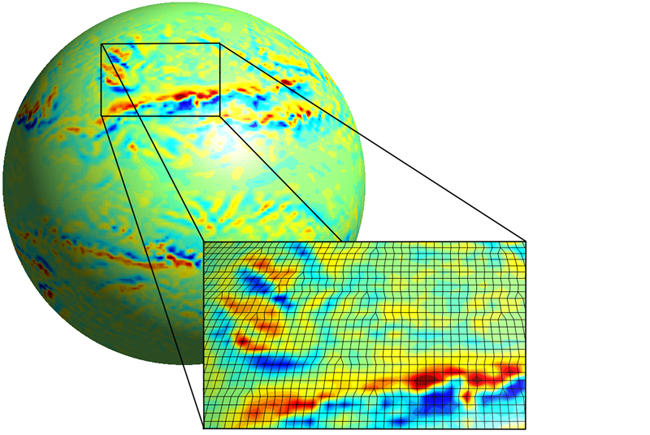
\includegraphics[width=8cm]{img/numerical_prediction_model.png}
  \caption{Príklad numerického modelu zameraného na meranie vertikálneho pohybu atmosféry}
  \label{numModel}
\end{figure}

\subsection{Počasie na Zemi}
Zem je treťou planétou v rámci Slnečnej sústavy, zároveň sa nachádza v pásme vhodného pre vznik života. Doba obehu okolo svojej materskej hviezdy trvá 365 dní, rotácia okolo svojej osi trvá 23.93 hodín. Zem je dosiaľ jediné známe teleso s tekutou vodou vhodnou pre život. Až 70 percent zemského povrchu tvorí voda.

Z pohľadu počasia sa Zem vyznačuje komplexnými poveternostnými systémami. Vietor môže dosahovať rýchlosť až 240 km/h vo forme triskových prúdov. Počasie podlieha ešte zložitejším javom z dôvodu interakcie oceánov a iných veľkých vodných plôch ako napríklad morí. Mraky tvorí vodná para zmiešavaná s ľadom. Práve rovnováha týchto dvoch prvkov spôsobuje atmosférický jav nazývaný zrážky. Zrážky môžu vznikať primárne dvomi procesmi. V trópoch, kde sa ľad v oblakoch nevyskytuje ide o spájanie kvapiek vody v oblakoch. Po čase sa kvapky stanú dostatočne ťažké na to, aby opäť padli na povrch Zeme. Druhým spôsobom je interakcia vodnej pary a ľadu severne od oblasti trópov. V tomto prípade ľadové častice majú nižší tlak nasýtených pár ako voda. Postupne sa takéto ľadové kvapôčky spájajú až kým nie je častica natoľko ťažká, aby opäť dopadla na povrch. Vtedy padá na povrch Zeme buď ako dážď alebo vo forme krupobitia.

Výkyvy teplôt sa na Zemi pohybujú od veľmi veľkých v suchom podnebí až po minimálne vo vlhkých oblastiach. V poslednej dobe sa pozornosť upriamuje na skleníkový efekt, ktorý sme ľudskou činnosťou na Zemi dostali až do neželaných hodnôt. Tento efekt však už od počiatku Zeme stál za zrodom života, nakoľko správne množstvo sklenníkových plynov ako napríklad CO2 otepluje atmosféru Zeme na tú teplotu, ktorá sa označuje ako vhodná pre život. Problémom tohto efektu je aktuálne fakt, že teplota vzrastá do hodnôt, ktoré sú pre život neprijateľne z opačného hladiska ako zamŕzanie a teda práve topenie a zvyšovanie globálnej teploty aj lokálnej teploty do hodnôt, ktoré sú pre organizmus nebezpečné.

\subsubsection{Atmosféra Zeme}
\label{atmosferaZeme}
\paragraph{Atmosféra}je plynný obal Zeme, ktorý je pútaný ťiažovou silou k nej a zároveň s ňou aj rotuje. Udávaná horná hranica je 35-40 tisíc kilometrov, avšak samotná vrstva spojito prechádza priamo do kozmického priestoru, preto nie je možné udať presnú hodnotu hranice. Atmosféra je dynamický systém, v ktorom prebiehajú neustále procesy, ktoré sú avšak z dlhodobého hľadiska v relatívnej rovnováhe. Práve v atmosfére sa odohrávajú všetky javy počasia. Taktiež vďačíme práve atmosfére za podmienky vhodné na život na našej planéte, nakoľko zabezpečuje hneď niekoľko dôležitých aspektov:
\begin{itemize}
  \item zjemňuje výkyvy teplôt
  \item chráni organizmy pre slnečným a kozmickým žiarením
  \item chráni povrch pred dopadom menších kozmických telies
  \item zabezpečuje základné podmienky pre život
\end{itemize}

\paragraph{Vývoj atmosféry} na Zemi súvisí s geologcikými a geochemickými procesmi, taktiež aj s existenciou živých organizmov na našej planéte. Súčasná atmosféra Zeme je výsledkom evolúcie, keď pred 4.6 miliardami rokov obsahovala primárne ľahké plyny ako vodík a jeho zlúčeniny (napríklad metán), hélium alebo neón, dnesná atmosféra obsahuje primárne tie plyny, ktoré nereagovali s vodou - oxid uhličitý, dusík a podobne. Atmosféra postupom času chladla, vodná para kondenzovala, čo viedlo k tvorbe oceánov. Oxid uhličitý sa z atmosféry uvolňoval do oceánov a hornín, kde sa viazal v uhličitanoch. Až rozvoj živých organizmov, ktoré v procese fotosyntézy uvolňovali kyslík do ovzdušia, spôsobil jeho hromadenie v atmosfére Zeme. Vďaka tomu sa začala formovať ozónovrstva Zeme, ktorá začala chrániť Zem pred účinkami slnečného ultrafialového žiarenia. Pokles oxidu uhličitého v ovzduší a postupné navyšovanie kyslíka spôsobili pokles skleníkového efektu a markantné zníženie teploty Zeme na úroveň prijateľnú pre život na povrchu. Práve tento krok nenastal, keď sa pozeráme na inú planétu slnečnej sústavy - Venušu. Atmosféra, ktorú poznáme dnes, označujeme ako atmosféra III a registrujeme ju v časovom horizonte asi 400 miliónov rokov. 
\paragraph{Atmosféra Zeme} sa skladá z asi 78 percent dusíka, 21 percent kyslíka, 0,9 percenta argónu a 0,1 percenta iných plynov. Stopové množstvá oxidu uhličitého, metánu, vodnej pary a neónu sú niektoré z ďalších plynov, ktoré tvoria zvyšných 0,1 percenta. Dusík je molekula, ktorá sa do atmosféry dostáva procesom biologického rozkladu alebo sopečnou činnosťou. Zároveň je pre život nevyhnutný, nakoľko sa viaže v bielkovinách. Kyslík sa dostáva do atmosféry fotosyntézou. Je nevyhnutným prvkom, vďaka ktorému môžeme dýchať, taktiež je potrebný na rôzne oxidačné procesy. Argón je plyn, ktorý sa do atmosféry dostáva rádioaktívnym rozpadom draslíka v zemskej kôre. 
Ďalším plyn, ktorý je pre život na našej planéte nevyhnutný je ozón. Vzniká ionizáciou vzduchu napríklad pri búrke alebo taktiež fotochemicky - pôsobením slnečného UV žiarenia. Táto látka, napriek tomu, že je pre živé organizmy jedovatá, vo vyšších polohách atmosféry je pre život klúčová. V rozmedzí 10-50 km sa sústreďuje až 90 percent ozónu, preto tejto časti atmosféry hovoríme aj ozonosféra. 
\begin{figure}[!htbp]
  \centering
  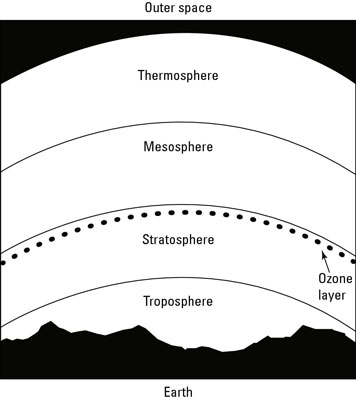
\includegraphics[width=8cm]{img/ozone.jpg}
  \caption{Ozónová vrstva Zeme}
  \label{numModel}
\end{figure}
\newline Dôvod, prečo je tento plyn jedným zo základným predpokladom života je fakt, že ozón pohlcuje UV žiarenie Slnka, ktoré má škodlivé účinky na živé organizmy. V podsledných desaťročiach sa často spomína pojem ozónová diera, ktorá má za následok úbytok ozónu v atmosfére a to len na niektorých, presne lokalizovaných miestach, väčšinou nad územím severného a južného pólu. Tento jav je pozorovaný približne od 80. rokov minulého storočia a môže zaň najmä freón - uhľovodík, ktorý nahrádza atóm kyslíka za halové prvky ako napríklad flór alebo bróm. Po týchto zisteniach sa upustilo od používania freónov, vďaka čomu nastal proces revitalizácie ozónovej vrstvy, ktorý by mal byť ukončený v roku 2050.

\paragraph{Rozdelenie atmosféry} sa uplatňuje z rôznych hľadísk. Prvým, ktorý opíšem sa určuje podľa zmeny teploty voči výške. Merania dokázali, že teplota s výškou klesá, avšak v niektorých častiach atmosféry teplota narastá. Toto zistenie viedlo k záveru, že atmosféra sa skladá z viacerých vrstiev vzduchu, pričom hlavné vrstvy sú oddelené od seba tenkými prechodnými vrstvami.
\begin{itemize}
  \item Troposféra - výška hranice sa pohybuje od 8 km nad pólmi až po 17 km smerom k rovníku. V troposfére je sustredených približne 80 percent vzduchu a prakticky všetká vodná para, taktiež práve v tomto rozmedzí prebiehajú všetky prírodné javy, ktoré nazývame počasie. Dôležitým pojmom v rámci tejto vrstvy je vertikálny teplotný gradient, ktorý udáva pokles teploty vo vertikálnom smere. Priemerná hodnota sa pohybuje približne v hodnote 0.65 °C na 100 m vertikálnej výšky.
  \item Tropopauza - prechodná vrstva medzi troposférov a stratosférou. Hrúbka tejto hranice predstavuje rádovo niekoľko sto metrov, v záležitosti od podmienok ale može predstavovať až hodnotu do 3 km. Teplotný rozsah sa pohybuje v hodnotách -50 až -80 °C. 
  \item Stratosféra - vrstva oddelená tropopauzou od troposféry siahajúca po výšku 55 km od hladiny mora. V tejto vrstve, narozdiel od troposféry, teplota s narastajúcou vertikálnou výškou stúpa a môže dosiahnuť až 0 °C v najvyšších polohách. Dôvodom sú prebiehajúce fotochemické reakcie sposobené vplyvom slnečného UV žiarenia, konkrétne rozkladom molekuly ozónu, ktorého sa v tejto vrstve nachádza až 90 percent z celkového objemu v atmosfére, preto sa táto oblasť nazýva aj ozónosféra. Koniec tejto vrstvy ohraničuje prechodová vrstva - stratopauza. 
  \item Mezosféra - nachádzajúca sa v rozmedzí 50 - 80 km, pričom teplota s výškou klesá až do -80 °C, zaujímavosťou je, že teplota klesá viac v lete ako v zime. Vo stúpajúcom vertikálnom smere ju následne oddeľuje mezopauza.
  \item Termosféra - vrstva siahajúca až do výšky 300 km, pričom pre posledných 100 km je význačný vzostup teploty s výškou, ktorá na konci predstavuje hodnotu až 1000 °C. V tejto vrstve je vzduch plne ionizovaný, teda obsahuje výhradne elektricky nabité častice. Práve z tejto oblasti je možné pozorovať žiaru meteorov v atmosfére. Taktiež je to oblasť, v ktorej je možné pozorovať polárnu žiaru, nakoľko sú práve v tejto vrstve ideálne podmienky na vstup nabitých častíc zo Slnka. Oddelujúca vrstva - termopauza sa uvádza ako oblasť, kde ešte tento jav môžeme pozorovať. 
  \item Exosféra - finálna časť atmosféry, ktorá už nemá konečné ohraničenie, teda voľne pokračuje do otvoreného kozmu. 
\end{itemize}

\begin{figure}[!htbp]
  \centering
  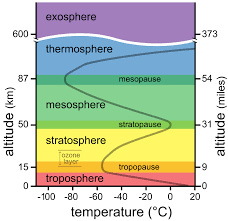
\includegraphics[width=8cm]{img/atmosphere.png}
  \caption{Atmosféra Zeme v závislosti s vývojom teploty}
  \label{numModel}
\end{figure}

Ďalším spôsobom členenia je podľa homogenity vzduchu: 
\begin{itemize}
  \item Homosféra - vertikálny priestor až do výšky 80 km od zemského povrchu. Zaraďujeme sem časti od tropsféry až po hranicu mezopauzi. Charakteristikou je, že v nej nepriebieha obmena zastúpenia zložiek vzduchu.
  \item Heterosféra - s hranicou od mezopauzi ide o časť, v ktorej sa znižuje koncentrácia ľahkých plynov so vzdialenosťou pomalšie ako koncentrácia ťažkých plynov. To je dôvod, prečo vo výške viac ako 1000 km od Zeme prevláda vodík. V tejto oblasti sa taktiež pozoruje priamy vplyv slnečného a kozmického žiarenia, čo spôsobuje napríklad aj jav fotoionizácie, ktorý zapríčiňuje zvýšenú teplotu v týchto oblastiach.
\end{itemize}

Taktiež je možné členenie podľa interakcie so zemským povrchom. Toto členenie je dôležité najmä kvôli zisťovaniu denných meteorologických údajov, pričom rozpoznávame rozdelenie na dve časti:

\begin{itemize}
  \item Hraničná vrstva atmosféry - v tejto časti sa výrazne prejavuje vplyv povrchu Zeme na prejav meteorologických údajov. Ohraničená je výškou, nad ktorou je už prúdenie vzduchu ovplyvnené len tiažovou silou, prípadne rozložením tlaku. Hranica taktiež záleží od reliéfu zemského povrchu, nad ktorou sa nachádza, pri členitejšom reliéfe sa nachádza vyššie ako pri rovinatom teréne. Všeobecne sa ale výška udáva v hodnotácha približne 1500 m. Nad touto úrovňou už nie je teplota vzduchu výrazne závislá od vplyvov zemského povrchu.
  \item Voľná atmosféra - nachádzajúca sa nad hraničnou vrstvou atmosféry. V tejto časti atmosféry už nemajú fyzikálne deje ani meteorologické vplyvy prakticky žiadny efekt.
\end{itemize}

\subsection{Mars}
Mars je štvrtou a zároveň poslednou planétou vnútornej sústavy planét slnečnej sústavy. Okolo Slnka obieha vo vzdialenosti 227 miliónov kilometrov a čas obehu okolo Slnka je 687 pozemských dní, čo predstavuje dĺžku dňa podobnú našej - 24.6 hodín. Okolo Marsu obiehaju dva malé satelity - Deimos a Phobos, asteroidy, ktoré boli gravitačnou silou Marsu vtiahnuté na jeho obežnú dráhu. Oba satelity sú oproti satelitu Zeme - Mesiacu mnohonásobne menšie s priemermi 11 a 22 metrov. \cite{} Teploty na Marse sú v priemere okolo -63 °C. Teploty sa však pohybujú od okolo -140 °C v zime na póloch až po 21 °C v nižších zemepisných šírkach v lete.

\subsubsection{Atmosféra Marsu}
\label{atmosferaMarsu}
Za posledné desaťročie bolo na povrch Marsu vypustených mnoho sond za účelom zistenia konzistencie povrchu. Ak by sme chceli prirovnať podmienky na Marse k tým na Zemi, najviac by sa povrch podobal púštným oblastiam. Povrch planéty je posiaty krátermi, ktoré boli vplyvom silného vetra na povrchu postupne uhladené a teda dnes vidíme len malé pozostatky. Práve vietor je jedným z primárnych atmosférických javov na povrchu planéty, nakoľko jeho pôsobením môžu nahromadené prvky podobné piesku vzniesť do ozvdušia a spôsobiť púštne búrky, ktoré sa v rámci roka dokonca na Marse periodicky opakujú. Následne môžeme občas dokonca aj z našej planéty za pomoci silnejšieho ďalekohľadu vidieť výraznejšie začervenanie planéty ako obvykle. Hornina, z ktorej je tento prach na povrchu Marsu zložený pozostáva najmä z danej červenkastej horniny, piesku a pôdy. V niektorých oblastiach Marsu sa vyskytujú miesta so zeleným zafarbením, avšak tento efekt nebol do dnešného dňa vysvetlený. Čo sa týka vody, známe sú ložiská vody pevného skupenstva na póloch planéty. Kvapalnú vodu sa nám do dnešného dňa nepodarilo objaviť napriek dôkazom erodovanej pôdy z plyvu práve vody kvapalného skupenstva. Taktiež sa predpokladá, že voda v kvapalnom skupenstve existuje aj pod povrchom Marsu, avšak vplyvom nízkeho atmosférického tlaku by sa voda vystupujúca na povrch ihneď pretvorila do plynného stavu. 
Atmosféra Marsu sa skladá predovšetkým z oxidu uhličitého. Avšak na rozdiel od Venuše je atmosféra Marsu veľmi tenká, vystavuje planétu bombardovaniu kozmickým žiarením a vytvára veľmi malý skleníkový efekt. Atmosférický tlak na povrchu Marsu je iba 1 až 2 percentá tlaku na Zemi. 
Tak ako na Zemi aj Mars má atmosféru a teda aj počasie. To, ako definujeme tieto dva pojmy na tejto planéte je však mimoriadne odlišné od toho, ako ich vnímame na našej planéte. Ako sme spomínali v sekcii \ref{atmosferaZeme}, Zemskú atmosféru tvorí asi 78 percent dusíka, 21 percent kyslíka, 0,9 percenta argónu a 0,1 percenta iných plynov. Taktiež obsahuje asi 1\% (backslash percent) vodnej pary. Atmosféra Marsu však pozostáva z 95\% (backslash percent) oxidu uhličitého, 3\% (backslash percent) dusíka, 1,6\% (backslash percent) argónu a obsahuje stopy kyslíka, oxidu uhoľnatého, prípadne vody. Vzduch na Marse je veľmi riedky a tlak v porovnaní je taktiež iba 1 až 2 percentá tlaku na Zemi. Pre predstavu, takýto tlak sa vyskytuje vo výške 45 kilometrov našej atmosféry. Tento tlak sa ešte mení s nadmorskou výškou, avšak stále pojednávame o veľmi malých, až zanedbateľných zmenách. Zaujímavosťou v rámci kolísania tlaku je však jeho periodické kolísanie v rámci sezóny. Je to z dôvodu vysokého množstva plynu CO2 v atmosfére, ktorý sa mení s ročnými obdobiami. Vyšší tlak sa vyskytuje počas južných letných mesiacov a najnižší počas severných letných mesiacov. Zmena je spôsobená rozdielom teplôt v danom období. Kým severné polárne zimy sú teplé a krátke, južné polárne zimy sú dlhšie a teplota klesá k nižším hodnotám. Práve južná polárna zima spôsobuje zamŕzanie plynu CO2 priamo v oblastiach južného pólu, čo spôsobuje pokles tohto plynu v atmosfére. Vtedy tlak na Marse klesá o približne 30 percent.
Cirkulácia atmosféry Marsiu je omnoho jednoduchšia ako na Zemi. V nižších zemepisných šírkach je dominantným javom pohyb Hadleyho buniek, ktoré predstavujú stúpajúci zohriaty vzduch v oblasti rovníka. Jedna časť prúdi na sever, druhá na juh do oblasti 30° zemepisnej šírky (do oboch smerov). Tam sa ochladzuje, klesá a prúdi opať k rovníku. V priamom toku zo severu na juh bráni rotácia planéty a reliéf Marsu. Vo vyšších zemepisných šírkach vznikajú polárne vzduchové masy, zároveň sa zo západu na východ tiahne séria oblastí vysokého a nízkeho tlaku. V týchto miestach v čase interakcii s Hadleyho bunkami môžu vznikach fronty počasia pretavujúce sa do búrok. Tie sú však v porovnaní s pozemskými omnoho pokojnejšie.
Veľký rozdiel Zeme a Marsu spočíva v tom, že Mars nemá žiadnu ozónovú vrstvu. Z toho vyplýva, že ultrafialové žiarenie zo Slnka nerušene dosahuje na povrch a teda škodlivo pôsobí na akékoľvek organické zlúčeniny na povrchu. Je to tiež dôvod, prečo atmosféra Marsu nemá žiadnu vrstvu zodpovedajúcej stratosfére Zeme, nakoľko by v takejto vrstve vysokonabité častice nemali s čím interagovať. 
Okrem vyššie spomínaných prašných búrok sa môžu vyskytovať na Marse aj oblaky zložené z ľadových častíc CO2, ktoré sa primárne sústreďujú v oblasti veľkých sopiek, kde sa najčastejšie tvoria vďaka dvíhaním častíc vetrom do vyšších oblastí, kde následne tieto častice kondenzujú. Taktiež sa môžeme stretnúť aj s takzvanými polárnymi kuklami - oblačnosti v polárnej oblasti, ktotér tvoria široké opary. Tento jav zachytilo už niekoľko pozemných roverov, ktoré zaznamenali sneženie počas chladných rán pred východom Slnka. 

\subsubsection{Ročné obdobia}
Teplota na Marse je oveľa nižšia ako na Zemi. Hlavné faktory, ktoré sa pod nízku teplotu podpisujú sú najmä vzdialenosť od Slnka a taktiež, ako sme spomínali vyššie, oveľa tenšia atmosféra tvorená prakticky výhradne oxidom uhličitým. Táto kombinácia faktorov robí z Marsu studený svet, kde môže teplota klesnúť až na hodnoty -120 °C, teda nižšie ako hodnoty namerané na našej planéte, kde sa podarilo doposiaľ namerať najnižšiu teplotu na úrovni -90 °C. V prípade najvyšších teplôt na Marse ide o hodnoty približne 20 °C. Táto teplota je výrazne nižšia v porovnaní s maximálnou nameranou teplotou na našej planéte, čo spôsobuje najmä tenká vrstva atmosféra, ktorá nie je schopná udržať tepelnú energiu. Aj preto sa priemerná hodnota teplôt na Marse stanovuje na úroveň -60 °C. Často je počas noci možné badať jav tvorenia mrazu na skalách, ktorý sa následne blížiacim úsvitom mení na paru, čím vzniká vlhkosť v ovzduší. Práve tento jav by v budúcnosti mohol prispieť k tomu, aby sa Mars stal obývateľnejším miestom. 
Podobne ako na Zemi, aj na Marse môžeme sledovať periodické striedanie štyroch ročných období, nakoľko sa planéta nakláňa okolo svojej osi. Tým, že excentricita planéty je výrazne väčšia ako Zeme, dĺžka ročných období je odlišná. Kým jar je na severnej pologuli najdlhším ročným obdobím s trvaním približne 7 pozemských mesiacov, leto a jesen zhodne trvajú približne 6 zemských mesiacov a zima ako najkratšie obdobie trvá približne 4 pozemské mesiace.
Každé ročné obdobie však trvá približne dvakrát dlhšie, pretože marťanský rok je približne dvakrát dlhší ako na Zemi. Mars obieha najbližšie k Slnku, keď je jeho južná pologuľa naklonená smerom k nemu, zatiaľ čo severná pologuľa je naklonená k Slnku, keď je od Slnka najďalej. Južné leto je preto oveľa teplejšie ako severné leto. Toto extra teplo prúdiace na južnú pologuľu spôsobuje väčšie turbulencie a poháňa silnejší vietor, ktorý vyvoláva najväčšie búrky. 
Pre jar na Marse je príznačné topenie oxidu uhličitého nahromadeného v polárnych častiach planéty. Táto pokrývka je sezónna a teda s rôznym ročným obdobím nadobúda oxid uhličitý uložený na týchto miestach rôzne skupenstvo.
\begin{figure}[!htbp]
  \centering
  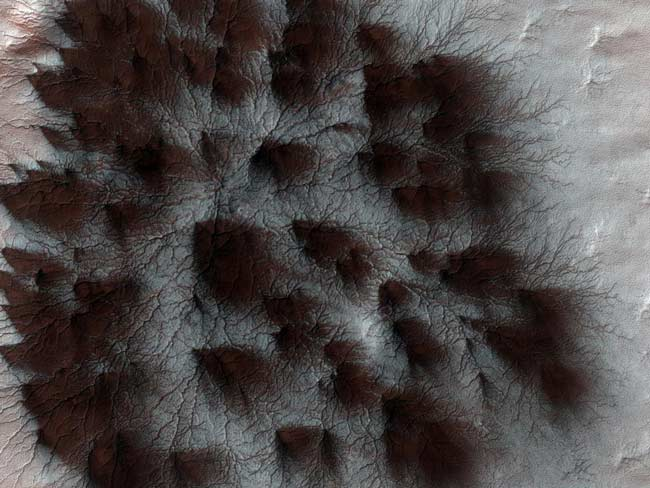
\includegraphics[width=8cm]{img/co2.jpg}
  \caption{Oxid uhličitý v pevnom skupenstve na povrchu Marsu}
  \label{co2}
\end{figure}
\newline Počas jari severná ľadová pokrývka sublimuje, pričom sa oxid uhličitý mení z pevného skupenstva priamo na plyn. To, koľko plynu sublimuje záleží od slnečného svetla, ktoré dopadá na danú oblasť. S pokračujúcou jarou všetok ľad v oblasti sublimuje, pričom plyn v atmosfére viaže na seba aj prachové častice. Akonáhle príde jeseň, polárna čiapočka tejto pologule začne opäť rásť. V lete severnej pologuli sa môžu vytvárať mraky, najmä okolo vrcholov sopiek. V iných obdobiach roka môže teplo stúpajúce z trópov, oblasti na oboch stranách rovníka, spôsobiť, že sa v tejto oblasti vytvorí oblačnosť, podobne ako na Zemi. Žiaden prachový oblak na Marse však neprodukuje dážď, hoci je možné, že sa na povrchu planéty môžu dočasne vytvoriť námrazy. Dokonca aj v lete je Mars so svojimi teplotami sotva obyvateľný, s minimami, ktoré dosahujú -140 °C. Občasné maximá však môžu vystúpať až k 20 °C.

\begin{table}[!htbp]
\caption{Dĺžka ročných období na Zemi a na Marse}
\centering
\begin{tabular}{lll}
Ročné obdobie & Dĺžka na Zemi & Dĺžka na Marse  \\
Jar           & 93            & 194             \\
Leto          & 93            & 178             \\
Jeseň         & 90            & 142             \\
Zima          & 89            & 154            
\end{tabular}
\end{table}
Počas obdobia marťanského leta je možné pozorovať úbytok polárnej ľadovej pokrývky, ktorá opäť narastá počas zimy. Práve pod touto vrstvou ľadu sú pravdepodobné ložiská tekutej vody.

Dôležitým parametrom, ktorý určuje dĺžku mesiacov ako na Marse tak aj na Zemi je poloha Slnka na nebeskej sfére pozdĺž ekliptiky z anglického Solar longitude, ktoré sa často skracuje len na Ls. Je to miera polohy telesa obiehajúceho na dráhe okolo Slnka, ktorá sa zvyčajne referenčne začína nulou v okamihu jarnej rovnodennosti. Práve vďaka tomuto parametru sme schopný merať čas tropického roka (rok ročných období) bez chýb, ktoré vychádzaju z kalendárneho určenia roka. Taktiež je to spôsom, ako môžeme opísať rok aj na iných planétach ako Zem, tada aj na Marse.
\begin{figure}[!htbp]
  \centering
  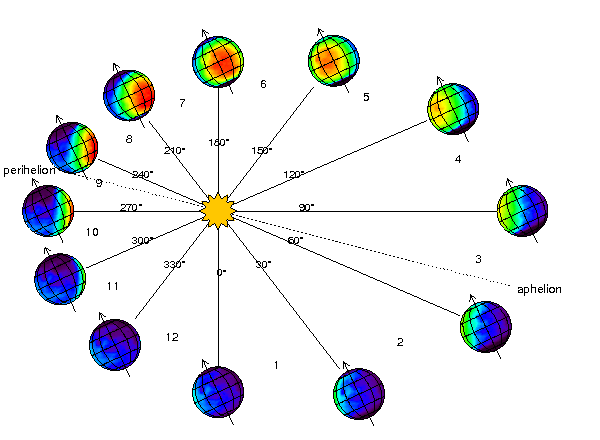
\includegraphics[width=8cm]{img/orbit.png}
  \caption{Uhol naklonenia Marsu voči Slnku v rámci jednej rotácie planéty}
  \label{solarLS}
\end{figure}

\begin{table}[!htbp]
\caption{Rozdelenie dĺžok mesiacov na Marse}
\centering
\begin{tabular}{llll}
Mesiac  & Ls (stupne)   & Sol            & Trvanie (dni)    \\
1       & 0 - 30        & 0.0 - 61.2     & 61.2             \\
2       & 30 - 60       & 61.2 - 126.6   & 65.4             \\
3       & 60 - 90       & 126.6 - 193.3  & 66.7             \\
4       & 90 - 120      & 193.3 - 257.8  & 64.5             \\
5       & 120 - 150     & 257.8 - 317.5  & 59.7             \\
6       & 150 - 180     & 317.5 - 371.9  & 54.4             \\
7       & 180 - 210     & 371.9 - 421.6  & 49.7             \\
8       & 210 - 240     & 421.6 - 468.5  & 46.9             \\
9       & 240 - 270     & 468.5 - 514.6  & 46.1             \\
10      & 270 - 300     & 514.6 - 562.0  & 47.4             \\
11      & 300 - 330     & 562.0 - 612.9  & 50.9             \\
12      & 330 - 360     & 612.9 - 668.6  & 55.7                                                     
\end{tabular}
\end{table}

\begin{table}[!htbp]
\caption{Udalosti na základe uhla naklonenia voči Slnku }
\centering
\begin{tabular}{lll}
Ls (stupne) & Udalosť                                       & Sezóna prachových búrok   \\
0           & Jarná rovnodennosť severnej pologule          & Koniec                    \\
71          & Aphelion (Najväčšia vzdialenosť Mars-Slnko)   &                           \\
90          & Letný slnovrat na severnej pologuli           &                           \\
180         & Jesenná rovnodennosť na severnej pologuli     & Začiatok                  \\
251         & Perihélium (najmenšia vzdialenosť Mars-Slnko) & Trvanie                   \\
270         & Zimný slnovrat na severnej pologuli           & Trvanie 
\end{tabular}
\end{table}

\newpage
\subsection{Existujúce riešenia}
Komplexný problém, akým predpoveď počasia nepochybne je by sa mohol na prvý pohľad zdať neriešiteľný z analytického pohľadu. Našťastie, existuje množstvo numerických algoritmov, ktorých cieľom je vyriešiť práve takéto typy problémov. 

Jedným z možných riešení, ktoré je dostupné na internete pojednáva problematiku predikcie meteorologických veličín, konkrétne teploty za pomoci strojového učenia a to rôznymi modelmi. Na testovanie si autori vybrali päť rôznych modelov: CNN, GRU, LSTM, Stacked LSTM, CNN-LSTM. Tieto modely natrénovali a následne sledovali výstupné parametre: RMSE, MSE a MAE. O týchto parametroch budem písať viac v praktickej časti. V princípe, proces predpovede spočíval v príprave dát, zvolení knižníc, zvolení premenných, riešení problému s chýbajúcimi dátami a rozdelením dát na časť trénovaciu a časť testovaciu. Následne nastal proces trénovania vyššie spomínanými modelmi, ktoré po natrénovaní vykazovali určité hodnoty parametrov RMSE, MSE a MAE. Z týchto údajov sa dalo usúdiť, že výsledný, ktoré najviac inklinovali k reálnym hodnotám poskytoval model LSTM. Táto informácia iba potvrdila naše domnienky zo štúdii týchto modelov, že práve model LSTM preukazuje pri danom probléme najlepšie výsledky. 

\subsection{Možnosti riešenia predpovede}
Zem je obalená atmosférou prevažne dusíka, kyslíka a vodnej pary. Vzduch pohybom priestorom nesie so sebou svoje vlastnosti a mení teplotu, vlhkosť, tlak a ostatné iné parametre a teda mení krátkodobý stav atmosféry - počasie. Počasie je teda vo svojej podstate vedľajším produktom našej atmosféry, ktorý prenáša teplo z jedného miesta na druhé.
Ako sme písali v podsekcii \ref{atmosferaZeme}, výkyvy počasia sa menia s lokáciou, kde na Zemi sa práve nachádzame. Taktiež, ako opisujeme v podsekcii \ref{atmosferaMarsu}, atmosféra na planéte Mars je výrazne pokojnejšia a teda zmena počasia je takmer úplne prepojená s ročným obdobím na planéte.
V tejto podsekcii chceme priblížiť vývoj predpovede počasia v histórii meraní.


\paragraph{Prvé zaznamenané merania} sú zaznamenané už v gréckymi filozofmi, ktorí položili základy vednej disciplíny, ktorú dnes nazývame meteorológia. Problémom doby bolo hlavne mylné chápanie prírodných javov, čo spôsobovalo následne zlý výklad vzťahov stavu počasia s rôznymi sprievodnými udalosťami. Pokrok nastal až vynálezom ortuťového barometra Evangelistom Torricellim, talianskym fyzikom a matematikom, ktorý v 17. storočí spôsobil revolúciu v tomto vednom odbore. Takmer palalne k tejto udalosti sa na svetlo sveta dostal aj prvý ortuťový teplomer, ktorý bol vytvorený na základoch objavu Galela Galileiho a jeho vynálezu plynného teplomera, ktorý napriek veľkej nepresnosti a teda nepoužiteľnosti v praxi slúžil ako predloha pre nový koncept s kvapalinou v skle.
17. a 18. storočie patrí medzi najdôležitejšiu etapu v posune meteorológii. Vďaka formulácii fyzikálnych zákonov tlaku plynu, teploty a hustoty od Roberta Boyla a Jacquesa Alexandra Cézara Charlesa, vývoju počtov od Isaaca Newtona a Wilhelma Leibniza, Daltonového zákona o parciálnych tlakoch zmesových plynov a mnohých ďalších zákonov bolo možné lepšie opísať a pochopiť dovtedy neznáme aspekty atmosféry. Následne 19. storočie prinieslo prvé výsledky a teda prvé užitočné predpovede počasia.

\paragraph{Analýza synoptických správ o počasí} započala vďaka výmene aktuálneho počasia na mnohých miestach Zeme. Veľmi dôležitým miľníkom bolo zostrojenie telegrafu, čo umožňovalo zhromažďovanie týchto údajov a ich výmenu prakticky po celom svete a tým vytvoriť mapu pozorovaní so vzorcami tlaku, vetra, teploty, oblačnosti a zrážok pri špecifickom čas. Od roku 1849 Joseph Henry vykresľoval denné mapy počasia na základe telegrafických správ a v roku 1869 Cleveland Abbe na Cincinnati Observatory začal poskytovať pravidelné predpovede počasia pomocou údajov získaných telegraficky.

\paragraph{Zriaďovanie sietí meteorologických staníc a služieb} viedlo k pravidelnej tvorbe synoptických máp počasia. Bolo to možné po tom, čo boli zorganizované siete staníc merania. Už od roku 1814 dostali pracovníci armádneho sektoru príkaz zaznamenávať údaje o počasí na svojich stanovištiach. Prvé siete meteostaníc začali vznikať prevažne v USA, Veľkej Británii a Holandsku. Postupne sa pridávali všetky veľkomestá po celom svete. Formy získavania dát boli rôzne, od bežných meteorologických staníc po sondy vysielané do atmosféry, aby z niekoľko kilometrovej výšky monitorovali stav. 

\paragraph{Moderné trendy a vývoj} technológií poskytlo prostriedky na testovanie nových vedeckých myšlienok. Koncom 20-tych a 30-tych rokov začalo niekoľko skupín vedcov získavať dáta za pomoci rádiovej komunikácie so sondami vo vyššej atmosfére Zeme. Tieto rádiosondy viedli k vzniku pozorovacích sietí vo vyšších častiach atmosféry. Pozorovania teploty a relatívnej vlhkosti pri rôznych tlakoch sú vysielané rádiom späť do stanice, z ktorej sú balóny vypúšťané a sledované radarmi a satelitmi globálneho pozičného systému za účelom zisťovania správania vetra.

\paragraph{Počas druhej svetovej vojny} zaznamenala meteorológia významný skok vďaka nasadeniu radara, ktorý poskytoval technológiu na monitorovanie búrok a pozorovanie štruktúr takejto oblačnosti. Moderné radarové systémy využívajú Dopplerov princíp frekvenčného posunu spojeného s pohybom smerom k alebo od radarového vysielača/prijímača na určenie rýchlosti vetra ako aj pohybu búrky.

\paragraph{Meteorologické merania zo satelitov a lietadiel} znamenal veľký prelom v meteorologických meraniach. Strednodobé predpovede, ktoré poskytujú informácie na päť až sedem dní vopred, ktoré boli predtým nemožné, začali satelity sprístupňovať globálne. Tieto predpovedné modely boli vyvinuté v americkom Národnom centre pre výskum atmosféry (NCAR), Európskom stredisku pre strednodobé predpovede počasia (ECMWF) a Národnom meteorologickom stredisku USA (NMC) a stali štandardom od 80. rokoch. Meteorologické satelity sa pohybujú po rôznych obežných dráhach a nesú širokú škálu senzorov. Sú dvoch základných typov: nízko letiaci polárny orbiter a geostacionárny orbiter. Kým prvý typ letí vo výške približne 700 kilometrov, druhý typ sa udržuje na orbite vo vzdialenosti približne 36 000 kilometrov. Práve technológia satelitov a celkovo vesmírneho inžinierstva nám umožnila aj tému tejto práce, ktorá pojednáva predikciu meteorologických veličín na inej planéte na základe údajov získavaných či už staticky z roverov na Marse alebo zo satelitov obiehajúcich okolo Marsu.





\subsection{Umelá inteligencia}
Spôsobov, ako definovať umelú inteligenciu je niekoľko. V princípe sa jedná o strojovú simuláciu procesov charakteristických pre ľudí a ich inteligenciu. Cieľom je, aby takto umelo vytvorená inteligencia bola schopná napodobňovať myseľ a činy ľudí. V konečnom dôsledku sa dá definovať umelá inteligencia ako technológia, ktorá stoje učí formou nadobúdania skúseností a prispôsobovaním sa novým vplyvom, prípadne učiť sa vykonávať repetitívne úlohy. V rámci repetitívnosti avšak narážame zároveň aj na definíciu hardvérom ovládanej robotickej automatizácie. Rozdiel spočíva v tom, že umelá inteligencia vykonáva takéto úlohy pomocou rôznych progresívnych algoritmoch učenia, čo spôsobuje jej nezávislosť od neustáleho ľudského zásahu.

Aplikácií pre umelú inteligenciu je neúrekom. Táto technológia môže byť použitá v rôznych sektoroch a odvetviach. Umelú inteligenciu testujeme a používame v zdravotníctve na liečbu u pacientov, predikciu vzniku nádorových ochorení alebo na chirurgické zákroky. Existujú počítače s umelou inteligenciou, ktoré hrajú šach alebo v dnešnej dobe veľmi rýchlo rozvíjajúci sa segment autonómneho riadenia áut. Pri každej z týchto aplikácii musíme zvážiť dôsledky akcie, pretože tieto akcie môžu ovplyvniť, v najhoršom prípade aj ohroziť život ľudí. Kým v šachu je konečným výsledkom víťazstvo v partii, pri autách s vlastným pohonom musí počítačový systém zohľadniť všetky externé údaje a konať tak, aby zabránil zrážke. Ďalším segmentom, kde umelá inteligencia má aplikácie je finančný priemysel, kde sa používa na zisťovanie aktivít v bankovníctve, napríklad nezvyčajné používanie debetných kariet alebo veľké vklady na účty – to všetko pomáha oddeleniu bankových podvodov. Používajú sa aj aplikácie pre umelú inteligenciu, ktoré pomáhajú zefektívniť a zjednodušiť obchodovanie. V neposlednom rade si aplikácie umelej inteligencie nachádzajú miesto aj v predpovediach budúcich udalostí a určovania vývoju na základe vstupov z minulosti. A práve túto vlastnosť chceme v tejto práci využiť a pokúsiť sa využiť aplikáciu predikcie počasia na základe časovej postupnosti meteorologických jednotiek.

Umelá inteligencia môže byť rozdelená do dvoch kategórií: slabá a silná. Slabá umelá inteligencia stelesňuje systém určený na vykonávanie jednej konkrétnej úlohy. Medzi tieto systémy umelej inteligencie patria napríklad hry alebo osobní asistenti. Silné systémy umelej inteligencie sú zase systémy, ktoré vykonávajú úlohy, ktoré sa svojou povahou približujú k tým, ktoré vykonávajú ľudia. Sú naprogramované tak, aby zvládli vyriešit situácie bez nutnosti zásahu ľudského faktora. Tieto druhy systémov možno nájsť v aplikáciách, ako je autonómna mobilita, vesmírny priemysel alebo v nemocničných aplikáciach.

Ďalšie rozdelenie umelej inteligencie zahŕňa oblasti vrátane počítačového programovania, strojového učenia, analytických modelov, spracovania prirodzeného jazyka, hlbokého učenia a neurónových sietí.

Na vývoj rôznych druhov umelej inteligencie sa píšu pokročilé algoritmy, ktoré sa kombinujú s cieľom rýchlejšej analýzy veľkých objemov údajov. Existuje niekoľko typov algoritmov umelej inteligencie, vrátane:
\paragraph{Regresné algoritmy} sa používajú, keď je cieľovým výstupom spojitá veličina. Počiatočný súbor dát musí mať označenia. Regresné algoritmy spadajú do kategórie kontrolovaného strojového učenia.

\paragraph{Klasifikačné algoritmy} prichádzajú do úvahy, ak je potrebné predpovedať výsledok na základe stanoveného počtu fixných, vopred definovaných výsledkov. Príklady zahŕňajú Naive Bayes, the Decision Tree, alebo Logistic Regression.

\paragraph{Algoritmy klastrovania} priraďujú vstupné údaje do dvoch alebo viacerých skupín na základe podobnosti rôznych vlastností. Je to forma strojového učenia bez dozoru, v ktorej sa algoritmus učí vzory z údajov bez označovania súboru dát.

Rôzne komponenty prispievajú k rôznym typom umelej inteligencie. Medzi prvky umelej inteligencie patria:
\paragraph{Strojové učenie} využíva štatistiku, fyziku a neurónové siete na získavanie poznatkov z údajov bez potreby toho, aby bol systém špecificky naprogramovaný na hľadanie v konkrétnej oblasti.

\paragraph{Neurónové siete} sú systémy strojového učenia, ktoré sa skladajú zo vzájomne prepojených jednotiek - neurónov. Neurónové siete spracovávajú informácie tak, že reagujú na externé vstupy a prenášajú informácie medzi jednotlivými jednotkami. Tento prístup im umožňuje vykonávať viacero prechodov v súbore dát tak, aby našli skryté spojenia.

\paragraph{Hlboké učenie} využíva mohutné neurónové siete s množstvom vrstiev, ktoré s dostatočným výpočtovým výkonom a vylepšenými tréningovými technikami umožňujú systémom identifikovať zložité trendy vo veľkom množstve údajov.

\paragraph{Počítačové videnie} využíva rozpoznávanie vzorov a hlboké učenie na spracovanie, analýzu a pochopenie obrázkov. Systémy dokážu zachytiť obrázky alebo video v reálnom čase a interpretovať ho.

\paragraph{Spracovanie prirodzeného jazyka} umožňuje počítačom analyzovať, porozumieť a vytvárať ľudský jazyk vrátane reči.

\subsection{Strojové učenie}
Strojové učenie je aplikácia umelej inteligencie, ktorá umožňuje systémom učiť sa a zlepšovať sa na základe skúseností bez toho, aby boli explicitne naprogramované. Strojové učenie sa zameriava na vývoj počítačových programov, ktoré majú prístup k dátam a používajú ich na učenie sa. Podobne ako ľudský mozog, ktorý získava vedomosti aj strojové učenie sa pri porozumení entitám spolieha na vstupy, ako sú tréningové údaje alebo znalostné grafy. S definovanými entitami môže začať hlboké učenie.
Proces strojového učenia sa začína pozorovaním alebo údajmi, ako sú príklady, historické údaje, priama skúsenosť alebo inštrukcie. Hľadá vzory v údajoch, aby mohol neskôr vyvodiť závery na základe poskytnutých príkladov. Primárnym cieľom ML je umožniť počítačom učiť sa bez nutnosti ľudského zásahu alebo asistencie a podľa toho prispôsobiť akcie.

Termín „strojové učenie“ zaviedol Arthur Samuel, počítačový vedec z IBM a priekopník v oblasti umelej inteligencie. Samuel navrhol počítačový program na hru dámy, ktorý čím viac hral, tým viac sa učil zo skúseností vďaka použitiu algoritmov na vytváranie predpovedí. Ako disciplína strojové učenie skúma analýzu a konštrukciu algoritmov, ktoré sa môžu učiť z dát a predpovedať ich. Vďaka obrovskému množstvu výpočtových schopností za úlohou alebo viacerými špecifickými úlohami možno stroje trénovať na identifikáciu vzorcov a vzťahov medzi vstupnými údajmi a automatizáciu procesov.

Systém učenia algoritmu strojového učenia môžeme rozdeliť na tri hlavné časti:
\begin{itemize}
    \item Rozhodovací proces: Vo všeobecnosti sa na predpovedanie alebo klasifikáciu používajú algoritmy strojového učenia. Na základe vstupných údajov, ktoré môžu byť označené alebo neoznačené algoritmus vytvorí odhad vzoru v dátach.
    \item Chybová funkcia: Chybová funkcia slúži na vyhodnotenie predpovede modelu. Ak existujú známe príklady, chybová funkcia môže vykonať porovnanie na posúdenie presnosti modelu.
    \item Proces optimalizácie modelu: Ak model môže lepšie zodpovedať dátovým bodom v trénovacej množine, potom sa váhy upravia tak, aby sa znížil nesúlad medzi známym príkladom a odhadom modelu. Algoritmus zopakuje tento proces vyhodnocovania a optimalizácie, pričom autonómne aktualizuje váhy, kým sa nedosiahne žiadaný prah presnosti.
\end{itemize}

Metódy strojového učenia môžeme rozdeliť na:
\paragraph{Učenie pod dohľadom} je definované používaním označených súborov dát na trénovanie algoritmov, ktoré presne klasifikujú údaje alebo predpovedajú výsledky. Keď sa vstupné údaje vkladajú do modelu, model prispôsobuje svoje hmotnosti, kým nie je model správne prispôsobený. Dochádza k tomu ako súčasť procesu krížovej validácie, ktorý zabezpečí vhodné prispôsobenie modelu. Niektoré metódy používané v kontrolovanom učení zahŕňajú neurónové siete, lineárnu regresiu alebo podporný vektorový stroj (SVM).

\paragraph{Učenie bez dozoru} využíva algoritmy strojového učenia na analýzu a zoskupovanie neoznačených množín údajov. Tieto algoritmy objavujú skryté vzory alebo zoskupenia údajov bez potreby ľudského zásahu. Jeho schopnosť objavovať podobnosti a rozdiely v informáciách z neho robí ideálne riešenie pre prieskumnú analýzu údajov, stratégie predaja, segmentáciu zákazníkov, rozpoznávanie obrazov a vzorov. Algoritmy používané v učení bez dozoru zahŕňajú neurónové siete alebo pravdepodobnostné metódy klastrovania.

\paragraph{Učenie sa čiastočne pod dohľadom} ponúka balans medzi učením pod dohľadom a učením bez dozoru. Počas tréningu používa menšiu označenú množinu dát na usmernenie klasifikácie a extrakcie funkcií z väčšej neoznačenej množiny údajov. Učenie s čiastočným dohľadom môže vyriešiť problém nedostatku označených údajov na trénovanie algoritmu učenia pod dohľadom.

Najčastejšie je možné nájsť aplikácie strojového učenia v rozpoznávaní reči, počítačovom videní, automatické obchodovanie alebo predikcie časových radov.

\subsection{Hlboké učenie}
Hlboké učenie je typ strojového učenia a umelej inteligencie, ktorý napodobňuje spôsob, akým ľudia získavajú určité typy vedomostí. Je dôležitým prvkom vedy o údajoch, ktorý zahŕňa štatistiku a prediktívne modelovanie. Je mimoriadne užitočný pre vedcov, ktorí majú za úlohu zbierať, analyzovať a interpretovať veľké množstvo údajov, nakoľko hlboké učenie robí tento proces rýchlejším a jednoduchším.
Hlboké učenie je možno považovať za spôsob automatizácie prediktívnej analýzy. Zatiaľ čo tradičné algoritmy strojového učenia sú lineárne, algoritmy hlbokého učenia sú usporiadané v hierarchii zvyšujúcej sa zložitosti a abstrakcie.
Aplikácie, ktoré využívajú hlboké učenie, prechádzajú takmer rovnakým procesom, ako človek, ktorý sa učí identifikovať objekt. Každý algoritmus v hierarchii aplikuje nelineárnu transformáciu na svoj vstup a používa to, čo sa naučí, na vytvorenie štatistického modelu ako výstup. Iterácie pokračujú, kým výstup nedosiahne prijateľnú úroveň presnosti. Práve veľký počet vrstiev spracovania údajov je inšpiráciou pre názov týchto typov siete.
V tradičnom strojovom učení je proces učenia pod dohľadom. Človek, ktorý pripravuje proces musí dbať na správny výber typov vecí, na ktoré sa má počítač zamerať. Pri tomto procese, ktorý sa nazýva extrakcia funkcii úspešnosť závisí od definície sady funkcii, ktoré boli použité. Pri hlbokom učení používame zostavovanie sád funkcii bez dozoru, teda programátor nemá nad procesom tvorby žiadny dosah. Takýto proces učenia sa ukázal ako rýchlejší a aj presnejší.
Na úvod procesu učenia sa môže použiť trénovacia množina údajov, ktoré vytvoria sadu funkcii a ktoré prispejú k zostaveniu prediktívneho modelu. S každou iteráciou, ktorou model prejde sa stáva nielen zložitejším ale aj presnejším. Na dosiahnutie prijateľne presného modelu je nutné poskytnúť modelu prístup k veľkému množstvu trénovacích údajov.
Na vytvorenie kvalitných modelov hlbokého učenia možno použiť rôzne metódy. Techniky zahŕňajú pokles rýchlosti učenia, prenos učenia alebo vypadnutie.
\paragraph{Pokles miery učenia} Rýchlosť učenia (learning rate) je hyperparameter – faktor, ktorý nastavuje podmienky pre jeho prevádzku pred procesom učenia. Zároveň riadi, akú veľkú zmenu model zažíva v reakcii na odhadovanú chybu pri každej zmene váh modelu. Príliš vysoké miery učenia môžu viesť k nestabilným tréningovým procesom alebo učeniu sa suboptimálnej sady váh. Príliš nízke miery učenia môžu spôsobiť zdĺhavý tréningový proces. Metóda poklesu rýchlosti učenia je proces prispôsobenia rýchlosti učenia na zvýšenie výkonu a skrátenie času tréningu.
\paragraph{Prenos učenia} Tento proces zahŕňa zdokonalenie predtým trénovaného modelu; vyžaduje rozhranie k vnútorným častiam už existujúcej siete. Po vykonaní úprav v sieti je možné vykonávať nové úlohy so špecifickejšími schopnosťami kategorizácie. Táto metóda má tú výhodu, že vyžaduje oveľa menej údajov ako iné, čím sa skracuje čas výpočtu na minúty alebo hodiny.
\paragraph{Dropout} Táto metóda rieši problém preťaženia v sieťach s veľkým množstvom parametrov náhodným vypustením jednotiek a ich spojení z neurónovej siete počas tréningu. Bolo dokázané, že táto metóda zlepšuje výkon neurónových sietí pri úlohách učenia s trénovacou množinou v mnohých oblastiach. 

Čo sa týka limitujúcich faktorov hlbokého učenia, veľké obmedzenie prichádza z dôvodu, že sa takéto siete učia pozorovaním. Znamená to, že sa učia to, čo vyplýva z údajov, ktoré do siete prichádzajú a na ktorých je sieť trénovaná. V prípade malého množstva alebo vysokej špecifičnosti údajov môžu modely dospieť do štádia trénovania, že ich nebude možné zovšeobecniť.


\subsubsection{Modely hlbokého učenia}

\subsubsection{Vrstvy hlbokého učenia}
Vrstva je stavebným kameňom najvyššej úrovne v hlbokom učení. Vrstva je kontajner, ktorý zvyčajne prijíma vážený vstup, transformuje ho množinou väčšinou nelineárnych funkcií a potom tieto hodnoty odovzdá ako výstup ďalšej vrstve. Vrstva je zvyčajne jednotná, to znamená, že obsahuje iba jeden typ aktivačnej funkcie, združovanie, konvolúciu atď., takže ju možno ľahko porovnávať s inými časťami siete. Prvá a posledná vrstva v sieti sa nazývajú vstupná a výstupná vrstva a všetky vrstvy medzi nimi sa nazývajú skryté vrstvy.

\subsubsubsection{Dense vrstva}

\subsubsubsection{LSTM vrstva}

\subsubsubsection{GRU vrstva}

\subsubsection{Hyperparametre hlbokého učenia}
\paragraph{Number of Hidden Layers}
\paragraph{Dropout}
\paragraph{Activation function}

\paragraph{Learning Rate}
\paragraph{Number of epochs}
\paragraph{Batch size}
\paragraph{Number of epochs}

\subsection{Výstupy a evaluácia výsledkov}

\paragraph{MAE} Stredná absolútna chyba je metrika hodnotenia modelu používaná v regresných modeloch. Stredná absolútna chyba modelu je priemer absolútnych hodnôt vzhľadom na testovaciu množinu jednotlivých chýb predikcie na všetkých inštanciách testovacej množiny. Každá chyba predpovede je rozdiel medzi skutočnou hodnotou a predpovedanou hodnotou pre inštanciu. \newline
$MAE = {\frac{1}{n}\sum_{i=1}^{n}(Y-\widehat{Y})}$

\paragraph{MSE} Stredná štvorcová chyba je metrika hodnotenia modelu, ktorá sa často používa pri regresných modeloch. Stredná štvorcová chyba modelu je priemerom štvorcových chýb predikcie vzhľadom na testovaciu množinu vo všetkých prípadoch v testovacej množiny. Chyba predikcie je rozdiel medzi skutočnou hodnotou a predpovedanou hodnotou pre inštanciu. \newline
$MSE = {\frac{1}{n}\sum_{i=1}^{n}(Y-\widehat{Y})^{2}}$

\paragraph{RMSE} Stredná kvadratická chyba je jedným z najčastejšie používaných meradiel na hodnotenie kvality predpovedí. Ukazuje, ako vzdialene predpovede padajú od skutočných nameraných hodnôt pomocou euklidovskej vzdialenosti. Na výpočet RMSE je nutné vypočítať tzv. reziduum, teda rozdiel medzi predpoveďou a pravdivou hodnotou pre každý dátový bod, vypočítať normu rezidua pre každý dátový bod, vypočítať priemer rezíduí a vypočítať druhú odmocninu tohto priemeru. RMSE sa bežne používa v aplikáciách, kde máme k dispozícii aj reálne dáta, nakoľko RMSE používa a potrebuje skutočné merania v každom predpovedanom údajovom bode. Pri strojovom učení je mimoriadne užitočné mať jedno číslo na posúdenie výkonu modelu, či už počas tréningu alebo validácie. RMSE je jedným z najpoužívanejších parametrov na tento účel. \newline
$RMSE = \sqrt{MSE} = \sqrt{\frac{1}{n}\sum_{i=1}^{n}(Y-\widehat{Y})^{2}}$


\newpage

\section{Praktická časť}

\subsection{Dáta}

\subsubsection{Dôležité parametre}
\subsubsection{Príprava dát}

\subsubsection{Implementácia}
\subsubsection{Typy neurónových sieti}
\subsubsection{Odskúšané modely}

\subsection{Výsledky}